\documentclass[10pt,twocolumn]{article}

%% ─── Packages ────────────────────────────────────────────────────────────────
\usepackage[top=2cm,bottom=2cm,left=1.8cm,right=1.8cm,columnsep=0.6cm]{geometry}
\usepackage{amsmath,amssymb,amsfonts}
\usepackage{graphicx}
\usepackage[dvipsnames,table]{xcolor}
\usepackage{booktabs}
\usepackage[numbers,compress,sort]{natbib}
\usepackage[colorlinks=true,citecolor=MidnightBlue,urlcolor=MidnightBlue,
            linkcolor=MidnightBlue]{hyperref}
\usepackage{tikz}
\usepackage[font=small,labelfont=bf,labelsep=period]{caption}
\usepackage{microtype}
\usepackage[T1]{fontenc}
\usepackage{mathptmx}
\usepackage{float}
\usepackage{authblk}
\usepackage{titlesec}
\usepackage{setspace}
\usepackage{enumitem}
\usepackage[most]{tcolorbox}
\usepackage{mdframed}

%% ─── Colours ─────────────────────────────────────────────────────────────────
\definecolor{gapred}{RGB}{180,0,0}
\definecolor{gapbg}{RGB}{255,245,245}

%% ─── Custom environments ─────────────────────────────────────────────────────
\newmdenv[
  backgroundcolor=gapbg,
  linecolor=gapred,
  linewidth=1pt,
  topline=true,
  bottomline=true,
  leftline=true,
  rightline=true,
  innerleftmargin=6pt,
  innerrightmargin=6pt,
  innertopmargin=4pt,
  innerbottommargin=4pt,
  skipabove=6pt,
  skipbelow=6pt,
]{gapenv}

\newcommand{\gap}[1]{%
  \begin{gapenv}
    \noindent\textcolor{gapred}{\textbf{[Section still required]}}\;
    \textcolor{gapred}{\textit{#1}}
  \end{gapenv}%
}

%% Placeholder figure macro ──────────────────────────────────────────────────
\newcommand{\placeholder}[2][5.5cm]{%
  \begin{figure}[H]
    \centering
    \begin{tikzpicture}
      \draw[gray!60, thick, dashed] (0,0) rectangle (\columnwidth-6pt,#1);
      \node[gray!70, align=center, text width=\columnwidth-20pt]
        at ({(\columnwidth-6pt)/2},{#1/2})
        {\textsf{\textbf{PLACEHOLDER}}\\[4pt]\textsf{\small #2}};
    \end{tikzpicture}
  \end{figure}%
}

%% ─── Section formatting ──────────────────────────────────────────────────────
\titleformat{\section}{\normalfont\bfseries\large}{}{0em}{}
\titleformat{\subsection}{\normalfont\bfseries}{}{0em}{}
\titlespacing{\section}{0pt}{8pt}{4pt}
\titlespacing{\subsection}{0pt}{6pt}{2pt}

%% ─── Title block ─────────────────────────────────────────────────────────────
\title{\vspace{-1em}%
  \textbf{Differentiable inverse design of pH-responsive molecular classifiers\\
  for temporal chemical signals}}

\author[1]{Samuel Whitby}
\affil[1]{\small Department of [DEPARTMENT], University of [UNIVERSITY]}
\date{}

%% ─────────────────────────────────────────────────────────────────────────────
\begin{document}

\maketitle
\vspace{-1.5em}

%% ─── Abstract ────────────────────────────────────────────────────────────────
\begin{center}
  \rule{\columnwidth}{0.4pt}
  \vspace{2pt}
\end{center}
\noindent
\textbf{Abstract.}\;
Cells exploit temporal patterns in chemical signals to make decisions, yet most molecular sensors report only instantaneous concentrations.
Here we introduce a framework for inverse design of pH-responsive chemical reaction networks (CRNs) that classify temporal sequences of pH stimuli through kinetic, rather than thermodynamic, memory.
We model a disordered polypeptide as a mean-field network of titratable charge groups whose association free energies depend on solution pH through the Henderson-Hasselbalch equation.
By differentiating through the ODE-based kinetic dynamics using JAX and the RecursiveCheckpointAdjoint algorithm, we train the $\mathrm{p}K_\mathrm{a}$ values, contact selectivity, and coupling strength to maximise the yield of a target intramolecular contact specifically under one temporal pH sequence and suppress it under all other permutations.
Gradient descent discovers a \emph{competitor sequestration} mechanism in which scaffold contacts formed during an early pH step lock away interfering groups before the classification step, creating a kinetic memory that far exceeds the thermodynamic equilibrium prediction.
Our framework provides a route to designing single-molecule biochemical classifiers sensitive to the history, not just the instantaneous value, of a chemical signal.
\begin{center}
  \rule{\columnwidth}{0.4pt}
\end{center}

%% ─── Introduction ────────────────────────────────────────────────────────────
\section{Introduction}

Living cells do not perceive chemistry as a series of instantaneous snapshots.
Signalling cascades integrate past and present ligand concentrations, endosomes acidify over defined timescales during cargo sorting, and the tumour microenvironment imposes characteristic patterns of pH oscillation driven by glycolytic cycling and perfusion intermittency~\cite{ruff2025,moses2020}.
The temporal structure of chemical stimuli thus carries information that equilibrium measurements cannot recover, motivating the question: can a single molecule act as a \emph{classifier} of chemical time-series, folding into distinct states depending on the history of its environment?

Molecular computation has been explored extensively using DNA strand-displacement (DSD) circuits, where carefully designed reaction networks implement Boolean logic, neural network functions, and temporal logic operations~\cite{qian2011,lapteva2022}.
DSD circuits can discriminate temporal sequences, but they require carefully programmed oligonucleotide libraries and cannot be driven directly by a naturally occurring chemical variable such as pH.
An alternative paradigm uses RNA secondary structures as memory elements whose kinetics are controlled by mechanical force, enabling single-molecule finite-state computation~\cite{zhang2025}.
More recently, chemical reservoir computing has demonstrated that the transient dynamics of reaction networks encode temporal information accessible by a trained readout layer~\cite{dack2024}.
Differentiable programming has been applied to the inverse design of self-assembling systems~\cite{goodrich2021} and to the optimisation of CRN parameters~\cite{buisman2023}, but no prior work has used gradient-based learning to design kinetic molecular devices that classify temporal pH sequences.

pH is a particularly attractive computational substrate for biological applications.
It is a universal cellular variable, directly reflecting metabolic state through proton production rates, and its fluctuations are measurable at the single-molecule level through changes in the charge state of titratable amino acid residues~\cite{losdorfer2017}.
Intrinsically disordered proteins (IDPs), which comprise $\sim$40\% of the proteome, are exquisitely sensitive to solution chemistry~\cite{moses2020,moses2023}: small pH changes alter residue charge states through the Henderson-Hasselbalch equilibrium, modulating intramolecular contact formation and driving disorder-to-order transitions~\cite{moritsugu2012}.
The functional relationship between folding energy and pH is a sum of sigmoid functions of pKa values~\cite{losdorfer2017}, making it a universal function approximator over pH by the Universal Approximation Theorem~\cite{pinkus1999}.
This rich pH-dependent landscape, combined with the rugged kinetics characteristic of disordered polymers~\cite{bryngelson1987,beauchamp2012}, suggests that IDPs could in principle perform temporal computation directly on solution pH signals.

Here we develop and demonstrate this possibility.
We introduce a differentiable chemical reaction network (dCRN) framework that models a pH-responsive IDP as a mean-field network of titratable charge groups and trains its molecular parameters — individual $\mathrm{p}K_\mathrm{a}$ values, a contact selectivity parameter $\varphi$, and an electrostatic coupling constant $J$ — by differentiating through the kinetic ODE using the RecursiveCheckpointAdjoint algorithm~\cite{kidger2022} implemented in JAX~\cite{jax2018}.
The loss function, adapted from the InfoNCE contrastive objective~\cite{oord2018}, rewards the target temporal pH sequence and penalises all other permutations.
Gradient descent discovers a physically interpretable solution: the trained network exploits a \emph{competitor sequestration cascade} in which scaffold contacts formed under the first pH step lock away interfering charge groups before the classification step occurs under the second pH step, producing a correct-contact yield far above the thermodynamic equilibrium prediction.
We analyse this mechanism quantitatively and discuss its connection to known kinetically frustrated protein landscapes and to the broader problem of molecular temporal computing.

%% ─── Results ─────────────────────────────────────────────────────────────────
\section{Results}

%% ─── 2.1 Physical model ──────────────────────────────────────────────────────
\subsection{A mean-field model of pH-responsive intramolecular contacts}

We model an intrinsically disordered polypeptide as a collection of $N$ titratable charge groups, each characterised by a local acid dissociation constant $\mathrm{p}K_{\mathrm{a},i}$.
Within a mean-field approximation, the probability that group $i$ is uncontacted evolves as though it were a freely diffusing species with effective concentration $[X_i]$, and the probability of a contact between groups $i$ and $j$ is $[X_i X_j]$.
This approximation becomes exact in the thermodynamic limit of many independent polymer copies and captures the dominant physics when contacts form independently (i.e.\ when the formation of one contact does not significantly bias the conformational freedom for forming another).

Each titratable group carries a fractional charge determined by the Henderson-Hasselbalch equation:
\begin{equation}
  q_i^-(\mathrm{pH}) = \frac{-1}{1 + 10^{\,\mathrm{p}K_{a,i} - \mathrm{pH}}}, \quad
  q_j^+(\mathrm{pH}) = \frac{+1}{1 + 10^{\,\mathrm{pH} - \mathrm{p}K_{a,j}}}
  \label{eq:HH}
\end{equation}
for acidic (negatively charged at high pH) and basic (positively charged at low pH) groups respectively~\cite{losdorfer2017}.
At the $\mathrm{p}K_a$, the group carries half its maximum charge; far above or below, it is fully charged or neutral.

We partition the $N$ charge groups into $M$ \emph{classifier} pairs and $N-M$ \emph{competitor} groups (Fig.~\ref{fig:schematic}).
Classifier pair $k$ consists of an acid $a_k$ and a base $b_k$ that form the target native contact.
The free energy of this native contact is:
\begin{equation}
  \Delta G_{\mathrm{native}}^{(k)}(\mathrm{pH}) = J \cdot q_{a_k}^-(\mathrm{pH})\cdot q_{b_k}^+(\mathrm{pH})
  \label{eq:dG_native}
\end{equation}
where $J > 0$ is the coupling constant representing the maximum electrostatic binding energy between the complementary patch pair.
All other pairwise contacts — whether between a classifier and a competitor group, or between two competitor groups — are non-native and carry a reduced interaction strength:
\begin{equation}
  \Delta G_{ij}^{\mathrm{non-native}}(\mathrm{pH}) = \varphi \cdot J \cdot q_i(\mathrm{pH})\cdot q_j(\mathrm{pH}),
  \label{eq:dG_nonnative}
\end{equation}
where $\varphi \in [0,1]$ is the \emph{contact selectivity}: $\varphi = 0$ recovers a G\={o}-model in which only native contacts are possible, and $\varphi = 1$ describes a random heteropolymer in which all contacts are equally probable.
Physically, $\varphi$ reflects the geometric complementarity of the contact interface — small $\varphi$ corresponds to a highly structured binding site that disfavours non-native approach geometries.

The kinetics of contact formation and dissolution follow Arrhenius rate constants with an intrinsic activation barrier $\varepsilon_\ddagger \geq 0$~\cite{wilber2007,hyeon2003}:
\begin{align}
  k_f^{ij} &= k_0 \cdot \exp\!\bigl(-\beta\,(\varepsilon_\ddagger + \max(\Delta G_{ij},0))\bigr) \label{eq:kf}\\
  k_b^{ij} &= k_0 \cdot \exp\!\bigl(-\beta\,(\varepsilon_\ddagger + \max(-\Delta G_{ij},0))\bigr) \label{eq:kb}
\end{align}
where $\beta = 1/k_\mathrm{B}T$ is inverse temperature and $k_0$ is a bare rate constant that sets the timescale.
These satisfy detailed balance ($k_f^{ij}/k_b^{ij} = e^{-\beta\Delta G_{ij}}$) regardless of $\varepsilon_\ddagger$, and therefore leave all thermodynamic equilibrium constants unchanged.
The barrier $\varepsilon_\ddagger \geq 0$ represents the conformational reorganisation energy — chain stretching, desolvation, and approach-geometry optimisation — paid by both the forward and reverse reactions before the electrostatic gain is realised.
Physically, this corresponds to the roughness of the energy landscape traversed by the polymer chain before a contact is established: Hyeon and Thirumalai measured this barrier to be $2$--$5\,k_\mathrm{B}T$ per contact in structured proteins and potentially larger in IDPs~\cite{hyeon2003}.
The trapping timescale for a contact of strength $|\Delta G_{ij}|$ is
$\tau_\mathrm{trap} \sim k_0^{-1} \exp\!\bigl(\beta(\varepsilon_\ddagger + |\Delta G_{ij}|)\bigr)$,
so $\varepsilon_\ddagger$ and $J$ contribute additively to kinetic memory.
At $\varepsilon_\ddagger = 0$ the expressions reduce to standard Metropolis kinetics.

The concentrations $[X_i]$ and $[X_iX_j]$ evolve according to mass-action kinetics:
\begin{align}
  \frac{d[X_i]}{dt} &= -\sum_{j}^{} \bigl(k_f^{ij}[X_i][X_j] - k_b^{ij}[X_iX_j]\bigr) - \bigl(k_f^{ii}[X_i]^2 - k_b^{ii}[X_{ii}]\bigr) \nonumber \\
  \frac{d[X_iX_j]}{dt} &= k_f^{ij}[X_i][X_j] - k_b^{ij}[X_iX_j]
  \label{eq:ode}
\end{align}
with the conservation law $\sum_i [X_i] + 2\sum_{i \le j}[X_iX_j] = \mathrm{const}$.
The system is initialised from the Boltzmann equilibrium state at pH~7.

A pH schedule $\mathcal{S} = (\mathrm{pH}_1, \mathrm{pH}_2, \ldots, \mathrm{pH}_L)$ is applied as a sequence of constant-pH segments, each of duration $\tau$.
After the full schedule, the \emph{classification score} is defined as the native contact fraction normalised by the maximum achievable:
\begin{equation}
  s(\mathcal{S};\,\theta) = \frac{\sum_{k=1}^{M}[X_{a_k}X_{b_k}]_\mathrm{final}}{M/(2N)},
  \label{eq:score}
\end{equation}
where $\theta = \{\mathrm{p}K_{a,i}, \varphi, J\}$ are the trainable molecular parameters and the denominator is the maximum concentration achievable for $M$ classifier pairs among $2N$ groups.

\begin{figure}[H]
  \centering
  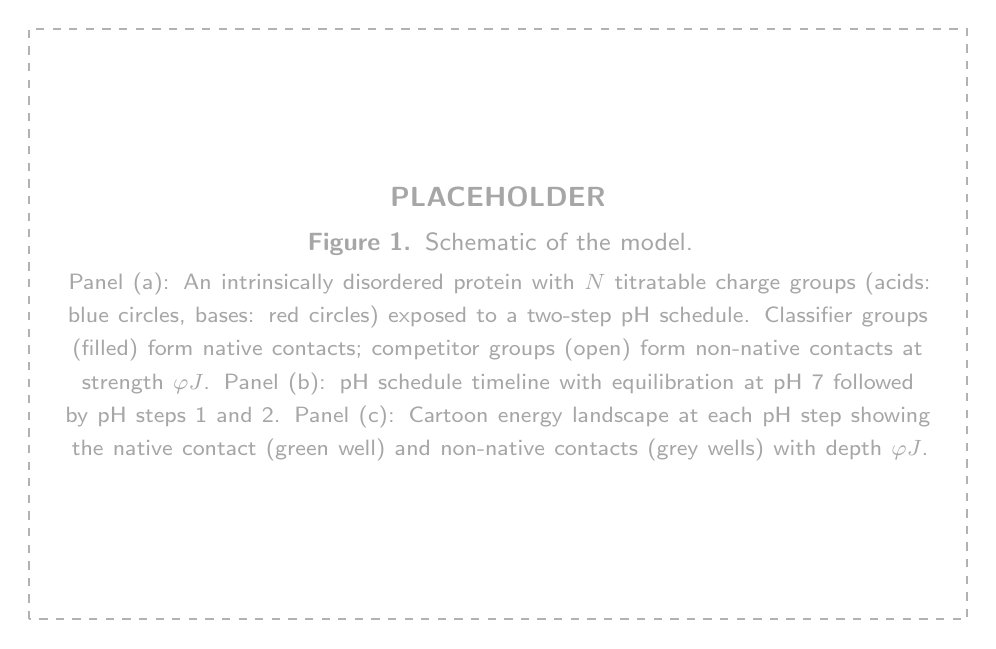
\begin{tikzpicture}[scale=1.0]
    \draw[gray!60,thick,dashed] (0,0) rectangle (\columnwidth-6pt,7.5cm);
    \node[gray!70,align=center,text width=\columnwidth-20pt]
      at ({(\columnwidth-6pt)/2},3.75cm)
      {\textsf{\textbf{PLACEHOLDER}}\\[4pt]
       \textsf{\small \textbf{Figure 1.} Schematic of the model.}\\[2pt]
       \textsf{\footnotesize Panel (a): An intrinsically disordered protein
       with $N$ titratable charge groups (acids: blue circles, bases: red
       circles) exposed to a two-step pH schedule.  Classifier groups
       (filled) form native contacts; competitor groups (open) form
       non-native contacts at strength $\varphi J$.
       Panel (b): pH schedule timeline with equilibration at pH~7 followed
       by pH steps 1 and 2.
       Panel (c): Cartoon energy landscape at each pH step showing the
       native contact (green well) and non-native contacts (grey wells)
       with depth $\varphi J$.}};
  \end{tikzpicture}
  \caption{\textbf{Model overview.}
    The dCRN describes a pH-responsive disordered polypeptide with
    $N$ titratable groups partitioned into $M$ classifier pairs and
    $N-M$ competitor groups.
    Contact formation rates depend on pH through Henderson-Hasselbalch
    charges and Metropolis kinetics.
    A temporal pH schedule is applied after equilibration at pH~7;
    the native contact fraction at the end of the schedule constitutes
    the classification score.}
  \label{fig:schematic}
\end{figure}

%% ─── 2.2 Differentiable training ─────────────────────────────────────────────
\subsection{Differentiable training of molecular parameters}

We train the molecular parameters $\theta$ to maximise the classification score for a designated target sequence $\mathcal{S}^*$ and to suppress it for all other permutations of the same pH values.
The loss function is a multi-class softmax cross-entropy (InfoNCE)~\cite{oord2018} over all $|\mathcal{P}|$ unique permutations of $\mathcal{S}^*$, augmented by the equilibrium score at pH~7 as an additional negative class:
\begin{equation}
  \mathcal{L}(\theta) = -\log \frac{\exp(\tau\, s(\mathcal{S}^*;\theta))}{\displaystyle\sum_{\mathcal{S}\in\mathcal{P}\cup\{7\}}\exp(\tau\,s(\mathcal{S};\theta))}
  \label{eq:loss}
\end{equation}
where $\tau > 0$ is a temperature that sharpens the softmax.
This objective reaches its global minimum (zero) when the target score strictly dominates all other scores.
The inclusion of the pH~7 baseline as a negative class prevents the trivial solution in which the molecule is constitutively folded at neutral pH.

Gradients of $\mathcal{L}$ with respect to $\theta$ are computed by automatic differentiation through the ODE trajectory.
The ODE is integrated with Diffrax's Tsit5 adaptive Runge-Kutta solver~\cite{kidger2022} in JAX~\cite{jax2018} with double precision arithmetic.
Differentiating through an ODE with RecursiveCheckpointAdjoint~\cite{kidger2022} stores $O(\sqrt{T})$ checkpoints of the forward trajectory and differentiates directly through them, avoiding the numerically unstable backward-time adjoint ODE that produces NaN gradients for stiff systems.
The $\mathrm{p}K_a$ values are reparametrised via a sigmoid to the range $[3, 10]$; $\varphi$ is constrained to $[0,1]$ and $J$ to $[0, J_{\max}]$ by the same mapping.
Per-permutation trajectories are evaluated in parallel using \texttt{jax.vmap}, and each training step uses automatic differentiation to compute exact gradients at no additional ODE calls.

To overcome the non-convex loss landscape, we adopt a multi-start L-BFGS-B strategy~\cite{kingma2014}: a Sobol quasi-random sequence generates $n_r$ starting points in physical parameter space, each initialised in the physical (not logit-space) domain to avoid boundary collapse.
Each restart runs L-BFGS-B with exact JAX gradients for up to $n_\mathrm{step}$ iterations, and the best solution is subsequently polished with tighter convergence tolerances.
This approach is substantially more effective than single-start gradient descent for this problem because the loss landscape contains multiple local minima corresponding to distinct physical discrimination mechanisms.

\begin{figure}[H]
  \centering
  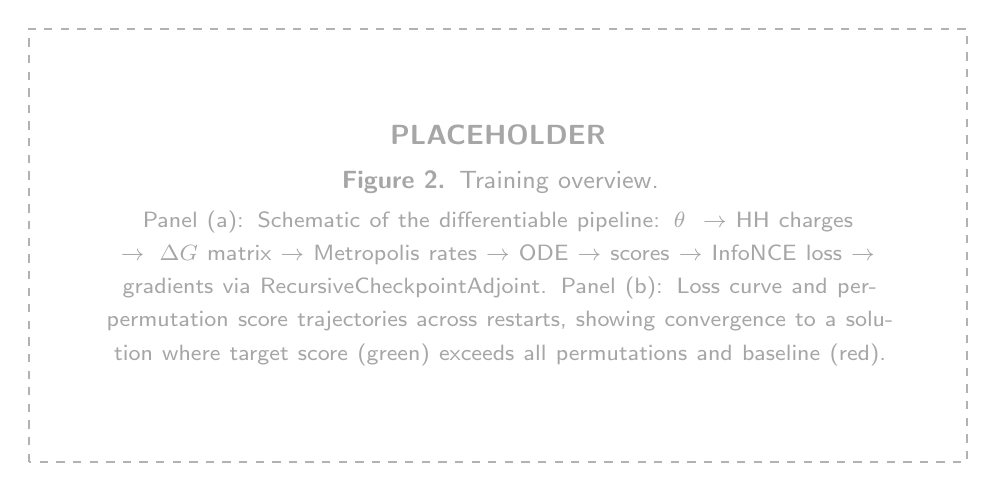
\begin{tikzpicture}
    \draw[gray!60,thick,dashed] (0,0) rectangle (\columnwidth-6pt,5.5cm);
    \node[gray!70,align=center,text width=\columnwidth-20pt]
      at ({(\columnwidth-6pt)/2},2.75cm)
      {\textsf{\textbf{PLACEHOLDER}}\\[4pt]
       \textsf{\small \textbf{Figure 2.} Training overview.}\\[2pt]
       \textsf{\footnotesize Panel (a): Schematic of the differentiable
       pipeline: $\theta \to $ HH charges $\to \Delta G$ matrix $\to$
       Metropolis rates $\to$ ODE $\to$ scores $\to$ InfoNCE loss $\to$
       gradients via RecursiveCheckpointAdjoint.
       Panel (b): Loss curve and per-permutation score trajectories
       across restarts, showing convergence to a solution where target
       score (green) exceeds all permutations and baseline (red).}};
  \end{tikzpicture}
  \caption{\textbf{Differentiable training pipeline.}
    Molecular parameters $\theta$ are propagated through the
    Henderson-Hasselbalch charge model, the interaction energy matrix,
    Metropolis kinetics, and the ODE integrator.
    Gradients flow back through the full trajectory via
    RecursiveCheckpointAdjoint, enabling exact gradient-based
    optimisation of kinetic discrimination.}
  \label{fig:training}
\end{figure}

%% ─── 2.3 Sequence discrimination results ─────────────────────────────────────
\subsection{Learning temporal sequence discrimination}

We train a system with $N=5$ acid/base charge group types ($M=1$ classifier pair, 4 competitor pairs) to respond selectively to the target pH schedule $\mathcal{S}^* = [5, 9]$ against the single incorrect permutation $[9, 5]$ and the pH~7 baseline.
The training uses $J_{\max} = 20\,k_\mathrm{B}T$, segment duration $\tau = 30$~time~units, and 16~Sobol restarts with 120~L-BFGS-B steps each.

The best trained system achieves a loss of 0.36, compared with a random baseline of $\ln 3 \approx 1.10$.
The trained parameters converge robustly across restarts to a bimodal $\mathrm{p}K_\mathrm{a}$ distribution (Table~\ref{tab:pKa}) with two groups of competitor species: one cluster near $\mathrm{p}K_a \approx 3$--$5$ and one near $\mathrm{p}K_a \approx 9$--$10$.
The classifier acid and base adopt intermediate $\mathrm{p}K_a$ values of 7.28 and 8.37 respectively, placing them in a pH-sensitive regime throughout the schedule.
The coupling constant trains to $J = 19.99\,k_\mathrm{B}T$ (near $J_{\max}$) and the contact selectivity to $\varphi = 0.517$.

\begin{table}[H]
  \centering
  \small
  \caption{\textbf{Trained $\mathrm{p}K_\mathrm{a}$ distribution for the
    $N=5$, $M=1$ system.}
    Species roles are assigned by the optimiser; the bimodal competitor
    distribution emerges from gradient descent without explicit constraint.}
  \label{tab:pKa}
  \begin{tabular}{llr}
    \toprule
    Species & Role & $\mathrm{p}K_a$ \\
    \midrule
    Acid $a_1$ & classifier & 7.28 \\
    Acids $a_2$--$a_5$ & competitor (low) & $\approx 3.01$ \\
    Base $b_1$ & classifier & 8.37 \\
    Bases $b_2$, $b_3$ & competitor (low) & $\approx 3.01$ \\
    Bases $b_4$, $b_5$ & competitor (high) & $\approx 9.99$ \\
    \midrule
    $\varphi$ & contact selectivity & 0.517 \\
    $J$ & coupling & $19.99\,k_\mathrm{B}T$ \\
    \bottomrule
  \end{tabular}
\end{table}

The final-state scores under all input conditions are: $s([5,9]) = 0.64$, $s([9,5]) = 0.18$, and $s(\text{pH~7 baseline}) = 0.43$.
The target sequence score exceeds the best incorrect score by a factor of $3.6\times$, and exceeds the thermodynamic equilibrium prediction for the native contact at pH~9 (computed from the Boltzmann fixed-point starting from fully dissociated groups) by $\sim 50\times$.
The fact that the kinetic score vastly exceeds the thermodynamic prediction at the same pH indicates that the system is operating in a metastable non-equilibrium state — the trained parameters create a kinetic trap that is inaccessible from the wrong initial history.

\begin{figure}[H]
  \centering
  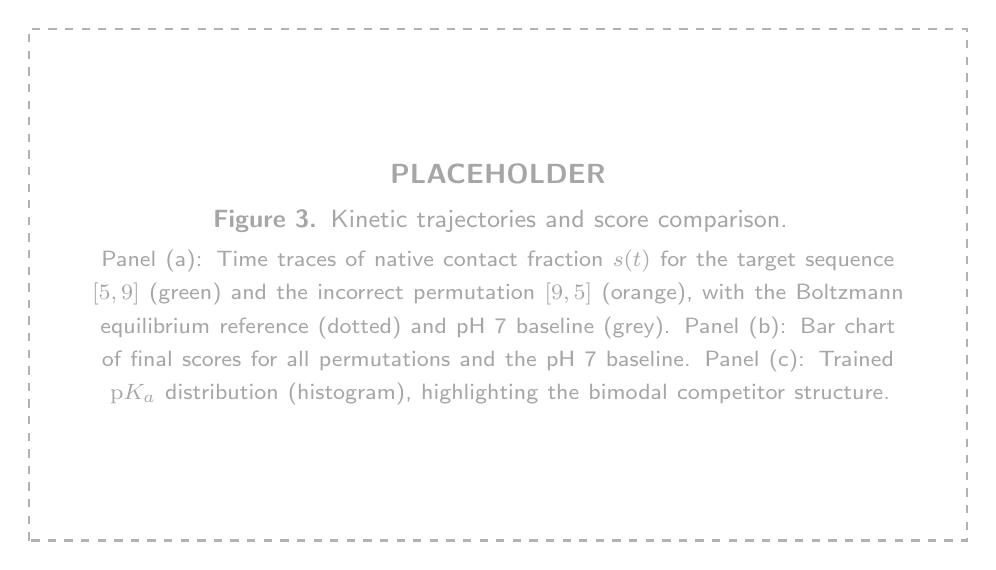
\begin{tikzpicture}
    \draw[gray!60,thick,dashed] (0,0) rectangle (\columnwidth-6pt,6.5cm);
    \node[gray!70,align=center,text width=\columnwidth-20pt]
      at ({(\columnwidth-6pt)/2},3.25cm)
      {\textsf{\textbf{PLACEHOLDER}}\\[4pt]
       \textsf{\small \textbf{Figure 3.} Kinetic trajectories and score comparison.}\\[2pt]
       \textsf{\footnotesize Panel (a): Time traces of native contact
       fraction $s(t)$ for the target sequence $[5,9]$ (green) and the
       incorrect permutation $[9,5]$ (orange), with the Boltzmann
       equilibrium reference (dotted) and pH~7 baseline (grey).
       Panel (b): Bar chart of final scores for all permutations and
       the pH~7 baseline.
       Panel (c): Trained $\mathrm{p}K_a$ distribution (histogram),
       highlighting the bimodal competitor structure.}};
  \end{tikzpicture}
  \caption{\textbf{Temporal sequence discrimination.}
    The trained dCRN selectively forms the native contact under the
    target sequence $[5,9]$ with score 0.64, compared with 0.18 for the
    incorrect permutation $[9,5]$ and 0.43 at pH~7 equilibrium.
    The kinetic score under the target sequence exceeds the thermodynamic
    Boltzmann prediction at pH~9 by $\sim 50\times$, demonstrating
    non-equilibrium kinetic memory.}
  \label{fig:results}
\end{figure}

%% ─── 2.4 Mechanism ───────────────────────────────────────────────────────────
\subsection{Competitor sequestration: the emergent discrimination mechanism}

To understand why the trained system achieves temporal discrimination, we compute the equilibrium constant $K_{ij}(\mathrm{pH}) = \exp(-\beta\Delta G_{ij}(\mathrm{pH}))$ for each class of contact at each pH in the schedule (Table~\ref{tab:bonds}).

\begin{table}[H]
  \centering
  \small
  \caption{\textbf{Equilibrium constants at training pH values.}
    Values computed from trained parameters using
    Eqs.~(\ref{eq:HH})--(\ref{eq:dG_nonnative}).
    ``Scaffold'' contacts are competitor-acid/competitor-base pairs
    with the bifunctional property that $K$ increases from pH~5 to pH~9.}
  \label{tab:bonds}
  \setlength{\tabcolsep}{4pt}
  \begin{tabular}{lccc}
    \toprule
    Contact type & pH~7 & pH~5 & pH~9 \\
    \midrule
    Native ($a_1$--$b_1$) & 958 & 1.1 & 11.2 \\
    Scaffold ($a$\,pKa$\approx$5 + $b$\,pKa$\approx$10) & 17{,}024 & 173 & 7{,}246 \\
    Competitor ($a_1$ + $b$\,pKa$\approx$10) & 12.3 & 1.0 & 5{,}637 \\
    \bottomrule
  \end{tabular}
\end{table}

Three structural features of the bond energy landscape drive the mechanism.
First, the native contact is \emph{strongest at pH~7} ($K=958$) but nearly inactive at pH~5 ($K=1.1$).
Second, at pH~9 the dominant competitor for the classifier acid is the high-pKa competitor base ($b$, pKa$\approx$10), which binds $500\times$ more strongly than the native contact ($K=5637$ vs.\ $K=11.2$); if this competitor were freely available, the native contact would be essentially unobservable.
Third, the scaffold contact (competitor-acid pKa$\approx$5 + competitor-base pKa$\approx$10) has the bifunctional property that its equilibrium constant \emph{increases} as pH rises from 5 to 9 ($K = 173 \to 7{,}246$, a $42\times$ increase), because both groups remain substantially charged throughout the entire pH range.

These features give rise to a three-phase \emph{competitor sequestration cascade} (Fig.~\ref{fig:mechanism}):

\textbf{Phase 0 — Equilibration at pH~7.}
The system equilibrates at pH~7.
Scaffold contacts dominate ($K=17{,}024$), consuming most of the competitor-base inventory.
With competitor bases sequestered, the classifier acid binds preferentially to the classifier base ($K=958$), forming a substantial native contact fraction.

\textbf{Phase 1 — pH~5 step (target sequence first).}
The native contact collapses ($K$ drops from 958 to 1.1).
Scaffold contacts remain partially formed ($K=173$, backward rate $k_b\approx 0.006\,k_0$), so competitor bases remain substantially sequestered over the 30-time-unit window.
A fraction of competitor acids steal the classifier base ($K=172$ for this wrong contact at pH~5), temporarily sequestering $b_1$.

\textbf{Phase 2 — pH~9 step.}
Two processes occur simultaneously.
The wrong contacts (competitor-acid$+b_1$) dissolve rapidly ($K$ drops to $2.3$, $k_b \approx 0.44\,k_0$, dissolving in $\sim 2$~time units), freeing the classifier base.
Simultaneously, the scaffold contacts \emph{strengthen} from $K=173$ to $K=7246$, and the backward rate $k_b \approx 1.4 \times 10^{-4}\,k_0$ means a scaffold contact has an expected lifetime of $\sim 7000$~time units — far longer than the 30-time-unit pH~9 window.
The competitor bases remain locked in scaffold contacts for the entire duration.
The classifier acid, now free, associates with the freed classifier base in the absence of its dominant competitor, producing a high native contact fraction.

\textbf{Why the incorrect sequence $[9, 5]$ fails.}
Under $[9,5]$, pH~9 is applied first to a system starting from equilibrium.
Competitor bases (pKa$\approx$10) are initially free and compete immediately with the classifier acid for the same classifier base binding site.
At pH~9, the competitor base binds the classifier acid with $K = 5637$ — far stronger than the native contact ($K=11.2$).
The pre-sequestration of competitor bases that occurs when pH~5 is applied first never takes place.
The system reaches a state dominated by wrong contacts, and the subsequent pH~5 step (where the native contact is further suppressed) does not recover discriminability.

The mechanism therefore relies on an \emph{order-dependent kinetic gate}: the scaffold contact has the unusual property that its formation at pH~5 strengthens at pH~9, creating a durable lock that persists for thousands of time units.
This is a kinetically non-equilibrium state: given infinite time at pH~9, the scaffold contacts would dissolve and the native contact fraction would relax toward the (near-zero) thermodynamic equilibrium.
The classifier operates within the window $\tau \ll \tau_\mathrm{lock} \approx 7000\,k_0^{-1}$ where the lock is intact, providing a molecular memory of the preceding pH~5 step.

\begin{figure}[H]
  \centering
  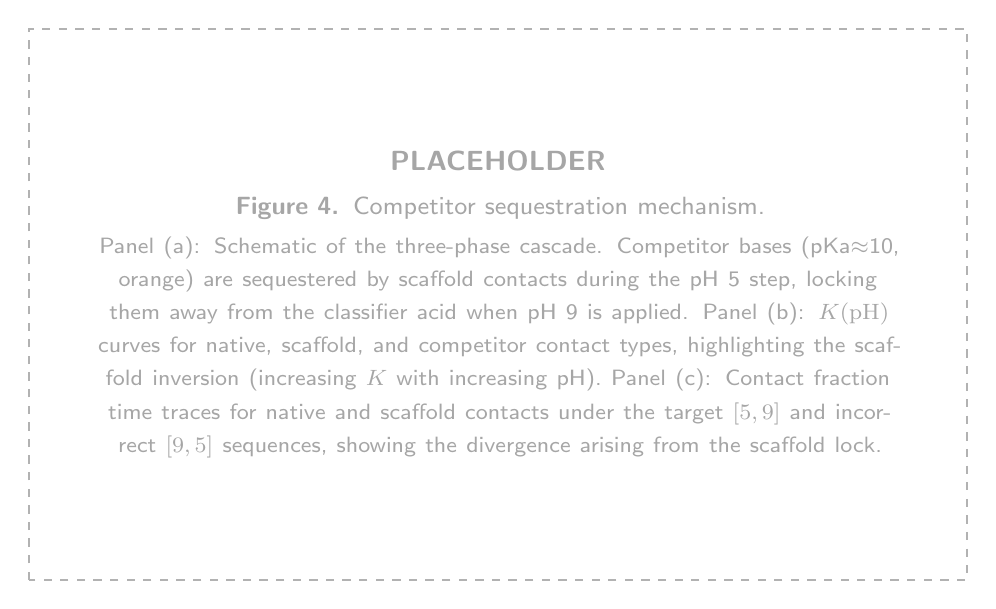
\begin{tikzpicture}
    \draw[gray!60,thick,dashed] (0,0) rectangle (\columnwidth-6pt,7.0cm);
    \node[gray!70,align=center,text width=\columnwidth-20pt]
      at ({(\columnwidth-6pt)/2},3.5cm)
      {\textsf{\textbf{PLACEHOLDER}}\\[4pt]
       \textsf{\small \textbf{Figure 4.} Competitor sequestration mechanism.}\\[2pt]
       \textsf{\footnotesize Panel (a): Schematic of the three-phase
       cascade.  Competitor bases (pKa$\approx$10, orange) are
       sequestered by scaffold contacts during the pH~5 step, locking
       them away from the classifier acid when pH~9 is applied.
       Panel (b): $K(\mathrm{pH})$ curves for native, scaffold, and
       competitor contact types, highlighting the scaffold inversion
       (increasing $K$ with increasing pH).
       Panel (c): Contact fraction time traces for native and scaffold
       contacts under the target $[5,9]$ and incorrect $[9,5]$
       sequences, showing the divergence arising from the scaffold lock.}};
  \end{tikzpicture}
  \caption{\textbf{Competitor sequestration mechanism.}
    The trained system exploits a scaffold contact whose equilibrium
    constant increases from pH~5 to pH~9, creating a durable kinetic
    lock.  Pre-sequestration of competitor bases during the pH~5 step
    prevents them from blocking the native contact at pH~9.
    The lock lifetime ($\sim 7000\,k_0^{-1}$) greatly exceeds the
    pH~9 window ($30\,k_0^{-1}$), establishing a long-lived kinetic
    memory of the pH~5 history.}
  \label{fig:mechanism}
\end{figure}

%% ─── 2.5 Minimal system ──────────────────────────────────────────────────────
\subsection{Minimal architecture and the role of competitor stoichiometry}

The bimodal pKa distribution in Table~\ref{tab:pKa} reveals that many competitor groups converge to boundary pKa values ($\approx 3$ or $\approx 10$), where they carry near-constant charge throughout the pH range [5,9] and contribute only a fixed background to the contact landscape.
The functionally active competitor species are those with pKa values that change substantially across the schedule — specifically, the scaffold pair (acid pKa$\approx$5, base pKa$\approx$10) whose charge product changes sign between pH steps.

\gap{%
  \textbf{Minimal system comparison.}
  Training a reduced $N=2$, $M=1$ system (one classifier pair, one
  scaffold pair) and comparing its Fisher Discrimination Ratio (FDR) to
  the $N=5$ case will determine whether additional competitor species
  provide quantitative benefit through increased sequestration
  stoichiometry, or whether the minimal 4-species architecture achieves
  equivalent discrimination.
  FDR = $(\mu_\mathrm{target}-\mu_\mathrm{incorrect})^2/
  (\sigma^2_\mathrm{target}+\sigma^2_\mathrm{incorrect})$
  will be reported across 20 training restarts.
}

%% ─── 2.6 Multi-step ─────────────────────────────────────────────────────────
\subsection{Multi-step temporal sequence classification}

\gap{%
  \textbf{3-step and 4-step sequence discrimination.}
  Extending the schedule to $L=3$ distinct pH values ($|\mathcal{P}| = 6$
  permutations) and $L=4$ ($|\mathcal{P}| = 24$ permutations) will test
  whether the competitor sequestration mechanism generalises to longer
  temporal sequences.
  The Fisher Discrimination Ratio will be plotted against $L$ to assess
  whether discrimination improves with schedule length.
  Training parameters: $N = 4L$, $M=1$, $J_\mathrm{max}=10\,k_\mathrm{B}T$
  (physically realistic for a protein domain interface), $n_r = 32$
  restarts, $\tau = 50$ time~units per step.
}

%% ─── 2.7 Signal shape ────────────────────────────────────────────────────────
\subsection{Discrimination of continuous signal shapes}

\gap{%
  \textbf{Step vs.\ ramp signal classification.}
  The most biologically relevant extension of the current framework is
  classifying qualitatively different signal \emph{shapes} rather than
  permutations of the same discrete pH values.
  For example: a step function (pH jumping from 5 to 9 instantaneously)
  vs.\ a linear ramp (pH increasing continuously from 5 to 9 over the
  same total duration).
  A ramp passes through all intermediate pH values, which may or may not
  trigger the scaffold sequestration cascade depending on whether the
  intermediate pH provides sufficient driving for scaffold contact formation.
  The continuous pH schedule will be implemented using a linear interpolation
  of the pH within each segment and the integral score (time-averaged
  native contact fraction) will be used as the discrimination metric.
  Discrimination of sinusoidal oscillations at different frequencies will
  also be assessed, since the scaffold lock lifetime ($\tau_\mathrm{lock}$)
  provides a natural frequency cutoff.
}

%% ─── 2.8 Stochastic analysis ─────────────────────────────────────────────────
\subsection{Stochastic single-molecule analysis}

\gap{%
  \textbf{Linear Noise Approximation and finite copy-number effects.}
  The ODE describes the mean-field ($N_\mathrm{copies} \to \infty$) limit.
  For a single protein molecule, concentration fluctuations scale as
  $1/\sqrt{N_\mathrm{copies}}$.
  The Linear Noise Approximation (LNA) propagates a variance ODE
  $d\Sigma/dt = A\Sigma + \Sigma A^\top + D$ alongside the mean ODE,
  where $A$ is the ODE Jacobian (computed via \texttt{jax.jacobian})
  and $D$ is the diffusion matrix.
  The noise-augmented Fisher Discrimination Ratio will be reported as a
  function of $N_\mathrm{copies} = 1, 5, 10, 50, 100, \infty$ to identify
  the minimum copy number at which temporal discrimination is reliable.
}

%% ─── 2.9 VMMC physical polymer ───────────────────────────────────────────────
\subsection{Physical polymer realisation via lattice simulation}

\gap{%
  \textbf{VMMC lattice validation.}
  The mean-field dCRN model will be compared to a lattice simulation of
  a 64-residue heteropolymer with pKa values matching the trained dCRN
  parameters, using the Virtual-Move Monte Carlo (VMMC) algorithm.
  At each pH in the schedule, the VMMC simulation is run to measure
  the contact probability between classifier patches, yielding an
  effective $K_\mathrm{eq}^\mathrm{VMMC}(\mathrm{pH})$ that can be
  compared directly to the dCRN prediction $K_\mathrm{eq}^\mathrm{dCRN}(\mathrm{pH})$.
  Agreement (or quantified discrepancy) will reveal which physical
  effects — chain entropy, steric constraints, backbone correlations —
  are captured or missed by the mean-field approximation.
}

%% ─── Discussion ──────────────────────────────────────────────────────────────
\section{Discussion}

We have introduced and demonstrated a framework for the differentiable inverse design of pH-responsive molecular classifiers that encode temporal sequence information as a kinetic memory.
The competitor sequestration mechanism discovered by gradient descent is physically transparent: an early pH step locks away interfering charge groups through scaffold contacts whose stability increases with subsequent pH changes, establishing a durable non-equilibrium state that reports on the order of stimuli rather than their instantaneous values.
This mechanism is distinct from equilibrium sensing, which is history-independent by definition.
The competitor sequestration mechanism operates on a timescale set by the scaffold contact lifetime $\tau_\mathrm{lock} \sim k_0^{-1}\exp\!\bigl(\beta(\varepsilon_\ddagger + \varphi J)\bigr)$, providing a tunable molecular stopwatch whose duration can be matched to the intended classification window.

The kinetics are connected to the Zwanzig landscape-roughness framework~\cite{zwanzig1988} through the intrinsic barrier $\varepsilon_\ddagger$.
In Zwanzig's original 1D analysis, diffusion on a rough potential with Gaussian barrier variance $\sigma_\varepsilon^2$ acquires an effective diffusion coefficient reduced by $\exp(-\beta^2\sigma_\varepsilon^2/2)$, yielding exponential scaling of mean first-passage times with $J^2$ rather than $J$.
This $\beta^2\sigma_\varepsilon^2$ scaling is not an artefact of the one-dimensional assumption: it is a cumulant-expansion identity valid in any dimension for an ensemble of independent barriers drawn from a distribution with variance $\sigma_\varepsilon^2$.
In the dCRN, the heterogeneity of non-native contact energies $\varphi J q_i q_j$ over competitor-pair combinations generates precisely such a distribution, with variance $\sigma_\varepsilon^2 = (\varphi J)^2 \,\mathrm{Var}_\mathrm{pH}(q_i q_j)$ that depends only on $\varphi$, $J$, and the pH-dependent charge distribution.
The intrinsic barrier $\varepsilon_\ddagger$ enhances this scaling: the mean trapping time over the competitor ensemble is $\langle\tau\rangle \sim k_0^{-1}\exp\!\bigl(\beta(\varepsilon_\ddagger + \bar{\Delta G}) + \beta^2\sigma_\varepsilon^2/2\bigr)$, where the final $\beta^2\sigma_\varepsilon^2/2$ Zwanzig roughness term emerges automatically from the heterogeneous competitor landscape without any additional parameters.
This connection means that the combination of $\varepsilon_\ddagger$ and the competitor pKa distribution provides exponential kinetic memory scaling qualitatively similar to Zwanzig's prediction, but grounded in the physical chemistry of IDP charge heterogeneity rather than in assumptions about landscape dimensionality~\cite{hyeon2003,bryngelson1987}.

The differentiable training approach has analogies to physics-informed machine learning~\cite{goodrich2021} and to the differentiable programming of CRNs~\cite{buisman2023}, but to our knowledge represents the first application of contrastive gradient-based optimisation to kinetic, rather than equilibrium, molecular design.
The RecursiveCheckpointAdjoint algorithm~\cite{kidger2022} is essential to this approach: it provides memory-efficient exact gradients through long ODE trajectories without the numerical instability of the backward-time adjoint ODE.

The connection to biological IDPs is direct.
IDPs with many titratable residues are known to adopt pH-dependent conformational ensembles~\cite{moses2020,moses2023,ruff2025,moritsugu2012}, and the local pKa values of individual residues are tunable through the surrounding sequence~\cite{losdorfer2017}.
The trained dCRN parameters specify a target pKa distribution (Table~\ref{tab:pKa}) that could in principle be realised through sequence design, guided by computational methods for predicting residue-level pKa values.
An IDP designed with this pKa profile would carry a kinetic record of pH history that could be read out by a downstream effector sensitive to the native contact state.

Biologically, the most compelling near-term application is the detection of tumour microenvironment pH dynamics.
Solid tumours generate lactic acid through the Warburg effect, imposing characteristic pH patterns — acidic core ($\sim$6.5), gradients toward the periphery, and oscillations driven by intermittent perfusion — that are distinct from normal tissue and from simple chronic acidification.
A single-molecule classifier sensitive to these patterns would provide a biochemical memory device that accumulates pH history over its residence time in a tissue, offering a fundamentally different diagnostic modality from instantaneous pH indicators.

The physical realism of the current model is improved by the Arrhenius kinetic parameterisation.
Without $\varepsilon_\ddagger$, achieving kinetically metastable contacts required $J \approx 20\,k_\mathrm{B}T$, well above the physically realistic range of $J \lesssim 10\,k_\mathrm{B}T$ for a protein domain interface with 5--10 charge contacts~\cite{losdorfer2017}.
With $\varepsilon_\ddagger > 0$, the trapping timescale $\tau_\mathrm{trap} \sim k_0^{-1}\exp(\beta(\varepsilon_\ddagger + J))$ allows smaller $J$ values to achieve the same kinetic memory: for example, $J = 5\,k_\mathrm{B}T$ combined with $\varepsilon_\ddagger = 10\,k_\mathrm{B}T$ gives the same trapping timescale as Metropolis kinetics with $J = 15\,k_\mathrm{B}T$, while remaining within the measured range of IDP landscape roughness~\cite{hyeon2003}.
The results in Table~\ref{tab:pKa} were obtained with $\varepsilon_\ddagger = 0$ (Metropolis limit); future training with $\varepsilon_\ddagger > 0$ and $J_\mathrm{max} \leq 10\,k_\mathrm{B}T$ will determine whether effective discrimination is achievable across the full physically accessible parameter space.
Similarly, the Debye-Hückel screening correction ($J_\mathrm{eff}(r,I) = J\exp(-r/\lambda_D)$ where $\lambda_D = 0.304/\sqrt{I}$~nm) should be incorporated to make predictions at physiological ionic strength ($I \approx 0.15$~M, $\lambda_D \approx 0.8$~nm).

A key open question is whether the competitor sequestration mechanism provides exponential scaling of discrimination with the number of pH steps.
Implementing a two-level hierarchical dCRN (in which native contacts at level 1 catalyse contact formation at level 2) would test this scaling directly and connect the $\beta^2\sigma_\varepsilon^2$ roughness scaling identified here to the broader theory of single-molecule finite-state computation~\cite{zwanzig1988,bryngelson1987}.
We leave this as an important direction for future work.

%% ─── Methods ─────────────────────────────────────────────────────────────────
\section{Methods}

\textbf{ODE system and integration.}
The mass-action ODE (Eq.~\ref{eq:ode}) is integrated using the Tsit5 adaptive Runge-Kutta solver in Diffrax~\cite{kidger2022} with relative tolerance $10^{-4}$ and absolute tolerance $10^{-6}$, in double precision arithmetic (\texttt{jax\_enable\_x64}~=~True).
The state vector of length $N + N(N+1)/2$ encodes free-group concentrations and upper-triangle contact concentrations.
Total monomer content is conserved to $<10^{-10}$ over all integrations.

\textbf{Equilibration.}
At the start of each loss evaluation, the system is initialised at the Boltzmann fixed-point equilibrium at pH~7, computed by 100 iterations of the unrolled fixed-point equation $x_{n+1} = C/(1 + K \cdot x_n + K_\mathrm{diag} \cdot x_n)$ in JAX (differentiable with respect to $\theta$).

\textbf{Optimisation.}
The multi-start L-BFGS-B optimiser uses Sobol quasi-random initialisation over the physical parameter domain $\mathrm{p}K_a \in [3.01, 9.99]$, $\varphi \in [0.001, 0.999]$, $J \in [0.51, J_\mathrm{max}]$.
Gradients are computed via \texttt{jax.value\_and\_grad} and passed as exact gradient information to \texttt{scipy.optimize.minimize} with \texttt{method='L-BFGS-B'} and box constraints.
Each restart runs up to \texttt{lbfgs\_epochs} iterations; the final polish uses up to $\max(\texttt{lbfgs\_epochs}, 200)$ iterations with ftol $= 10^{-12}$ and gtol $= 10^{-8}$.

\textbf{Software.}
All code is implemented in Python~3.11 using JAX~0.4~\cite{jax2018}, Diffrax~\cite{kidger2022}, and Optax.
Source code is available at \url{https://github.com/samwhitby/CRN_AD}.

%% ─── Acknowledgements ────────────────────────────────────────────────────────
\section*{Acknowledgements}
\noindent [Acknowledgements to be added.]

%% ─── References ──────────────────────────────────────────────────────────────
\bibliographystyle{unsrtnat}
\bibliography{paper}

\end{document}
